

%%%%%%%%%%%%%%%%%%%%%%%%%%%%%%%%%%%%%%%%%%%%%%%%%%%%%%%%%%%%%%%%%%%%%%%%
%    INSTITUTE OF PHYSICS PUBLISHING                                   %
%                                                                      %
%   `Preparing an article for publication in an Institute of Physics   %
%    Publishing journal using LaTeX'                                   %
%                                                                      %
%    LaTeX source code `ioplau2e.tex' used to generate `author         %
%    guidelines', the documentation explaining and demonstrating use   %
%    of the Institute of Physics Publishing LaTeX preprint files       %
%    `iopart.cls, iopart12.clo and iopart10.clo'.                      %
%                                                                      %
%    `ioplau2e.tex' itself uses LaTeX with `iopart.cls'                %
%                                                                      %
%%%%%%%%%%%%%%%%%%%%%%%%%%%%%%%%%%
%
%
% First we have a character check
%
% ! exclamation mark    " double quote  
% # hash                ` opening quote (grave)
% & ampersand           ' closing quote (acute)
% $ dollar              % percent       
% ( open parenthesis    ) close paren.  
% - hyphen              = equals sign
% | vertical bar        ~ tilde         
% @ at sign             _ underscore
% { open curly brace    } close curly   
% [ open square         ] close square bracket
% + plus sign           ; semi-colon    
% * asterisk            : colon
% < open angle bracket  > close angle   
% , comma               . full stop
% ? question mark       / forward slash 
% \ backslash           ^ circumflex
%
% ABCDEFGHIJKLMNOPQRSTUVWXYZ 
% abcdefghijklmnopqrstuvwxyz 
% 1234567890
%
%%%%%%%%%%%%%%%%%%%%%%%%%%%%%%%%%%%%%%%%%%%%%%%%%%%%%%%%%%%%%%%%%%%
%
% \documentclass[twocolumn,11pt,a4paper]{article}		%<-use this for checking equation length
\documentclass[12pt]{iopart} 

%<-comment out this for checking equations (author list too)
\usepackage{iopams,setstack} 

%<-comment out this for checking equations
\usepackage{graphicx, algorithm, algorithmicx, algpseudocode,epsfig} 
\usepackage{color} 
\usepackage[tight,scriptsize]{subfigure}

%\renewcommand{\subcapsize}{\small}
% \usepackage{anysize}							%<-use this for checking equation length
% \marginsize{1.7cm}{1.5cm}{0.3cm}{0.8cm}			%<-use this for checking equation length
% \setlength{\columnsep}{0.5cm}					%<-use this for checking equation length
% \usepackage{amsmath,amssymb,amsfonts} 			%<-use this for checking equation length
\newcommand{\todo}[1]{\textsf{\emph{\textbf{\textcolor{blue}{#1}}}}} 
\newcommand{\wtf}[1]{\textsf{\emph{\textbf{\textcolor{red}{#1}}}}} 
\newcommand{\omg}[1]{\textsf{\emph{\textbf{\textcolor{green}{#1}}}}} \begin{document}

\title[State and Parameter Estimation for Spatio-Temporal Neural Fields]{State and Parameter Estimation for Spatio-Temporal Neural Fields}

\author{Dean R. Freestone$^1$, Parham Aram$^2$, Michael Dewar$^3$, Kenneth Scerri$^4$, David B. Grayden$^1$, and Visakan Kadirkamanathan$^2$}

\address{$^1$ Department of Electrical and Electronic Engineering, University of Melbourne, Melbourne, Vic, 3010 Australia} \address{$^2$ Department of Automatic Control and Systems Engineering, University of Sheffield, Mappin Street, Sheffield, S1 3JD, UK} \address{$^3$ Department of Applied Physics and Applied Mathematics, Columbia University, US} \address{$^4$ Ken's} \ead{dfreestone@bionicear.org} 
\begin{abstract}
	Will do the abstract towards the end. 
\end{abstract}

%Uncomment for PACS numbers title message
%\pacs{00.00, 20.00, 42.10}
% Keywords required only for MST, PB, PMB, PM, JOA, JOB? 
%\vspace{2pc}
%\noindent{\it Keywords}: Article preparation, IOP journals
% Uncomment for Submitted to journal title message
%\submitto{\JPA}
% Comment out if separate title page not required
\maketitle

\section{Introduction} This paper presents a framework for creating patient specific macroscopic neural field continuum mathematical models. \todo{I think it's probably good to start like this, but there either needs to be more here or this needs to be folded into the following paragraph. Otherwise this first sentence looks a little out of place.}

The human brain is composed of approximately 100 billion neurons and 60 trillion synapses operating in concert and, despite decades of research, our understanding of neural dynamics remains modest. Hence research has focused on different scales of dynamics: from individual proteins, synapses, and neurons; to neuronal networks and ensembles of neuronal networks. While our understanding of the function of neurons is well developed, the overall behaviour of the brain's meso and macro-scale dynamics remains largely a mystery. Understanding the brain at this level is extremely important since this is the scale where pathologies such as epilepsy, Parkinson's disease and schizophrenia are manifested.

There has been much interest in generating physiologically plausible neural field models to study brain dynamics at the meso/macroscopic scale. Mathematical neural field models provide insights into the underlying physics and dynamics of electroencephalography (EEG) and magnetoencephalography (MEG) (see \cite{Deco2008} \cite{David2003} for recent reviews). These models have demonstrated possible mechanisms for the genesis of neural rhythms (such as the alpha and gamma rhythms) \cite{Liley1999} \cite{RENNIE2000}, epileptic seizure generation \cite{DaSilva2003}, \cite{Suffczynski2004} and \cite{Wendling2005} and insights into other pathologies \cite{Moran2008} \cite{Schiff2009} that would be difficult to gain from experimental data alone. 

Unfortunately, the use of these models in the clinic has been limited, since they are constructed for ``general'' brain dynamics whereas pathologies almost always have unique underlying patient specific causes. Patient specific data from EEG is readily available in the clinical setting, suggesting an opportunity to make the patient-specific link to models of cortical dynamics. However the meso/macroscopic neural dynamic state is not directly observable in EEG data, making predictions of the underlying physiology inherently difficult.

For models to be clinically viable they must be patient specific. A possible approach to achieve this would be to fit a general neural field model, like the Wilson and Cohen (WC) \cite{Wilson1973} model or a neural mass model like the Jansen and Ritt model \cite{Jansen1995}, to patient specific EEG data. Fitting the neural models to individuals is a highly non-trivial task, and until very recently this has not been reported in the literature. 

An estimation framework for neural field models known as dynamical causal modelling (DCM) \cite{David2003} \cite{David2006} has recently been proposed for studying evoked potential dynamics. Via a Bayesian inference scheme, DCM estimates the long range connectivity structure between the specific isolated brain regions that best explains a given data set. The interconnected brain regions are modelled by the Jansen and Ritt equations. Another recent publication describing a parameter estimation method with a neural field model used an Unscented Kalman filter with the WC neural field equations \cite{schiff2008kalman}. This work takes a system theoretic approach to the neural estimation problem and marks a first step in what has the potential to revolutionise the treatment of many neurological diseases where therapeutic electrical stimulation is viable.

Generating patient specific models allows the application of a range of techniques from control systems theory, where tailored electrical stimulation could be used therapeutically in a closed loop fashion. Currently available epileptic seizure  control devices (i.e., the vagal nerve stimulator) are implemented in an ``open loop". That is, the therapeutic electrical stimulation waveforms are adjusted for each patient by trial and error, disregarding the patient's neurodynamics and information about their particular pathologies. Given access to an accurate model, the application of optimal control theory in these circumstances would allow for robust therapeutic stimulations.

The work from Schiff and Sauer \cite{schiff2008kalman} successfully demonstrated it is possible to estimate parameters \wtf{what kind of parameters?} from the WC equations. This motivates the question, what parameters are the most important? How patient specific do the assumed parameters have to be for the model to be useful? In this paper, we address both of these questions and provide a theoretical platform to perform patient-specific grey-box modelling of the human neocortex. \wtf{not sure about rhetorical questions as a narrative mechanism in general, also not sure how this paper addresses these particular questions.} \omg{Maybe the next section addresses that the connectivity is important. Needs sharpening.}

\section{The Importance of Cortical Structure} Neural field models relate mean firing rates of pre-synaptic neural populations to post-synaptic mean membrane potentials. Each neural population represents a functional cortical processing unit, referred to as a column. The columnar organization of the cortex is continuous, where pyramidal cells are members of many columns. In general, cortical structure can be modeled in a physiologically plausible manner as being locally homogeneous (in short range intracortical connectivity) and heterogeneous (in long range cortico-cortical and corticothalamic connectivity) \cite{Jirsa2009} \cite{Qubbaj2007}. Locally, each column is thought be connected via symmetric short range local excitation, with surround inhibition \cite{Braitenberg1998}. For example, this structural organisation is most studied in the visual system, where the surrounding inhibition effectively tunes a cortical column to a particular receptive visual field \cite{Sullivan2006}.

Recent studies using neural field models have demonstrated the theoretical implications of specific connectivity structure of the cortical columns in neural field models, where the connectivity kernel governs the bifurcation points of the system \cite{Hutt2005} and types of oscillations that can be generated \cite{Schmidt2009}. This implies that if we could estimate the connectivity structure for an individual, then we could capture patient specific neurodynamics that lead to various oscillatory states. 

Estimating functional cortical connectivity via EEG promises to shed light on the hierarchy of brain regions that are involved in specific tasks, motivating the use of techniques like DCM. Other comparable methods are based on auto-regressive (AR) modelling of the EEG, MEG, or fMRI times series \todo{[refs!]}. Studies have concentrated on finding functional connectivity patterns using information contained in the AR coefficients using techniques like Granger causality \cite{Hesse2003}, the direct transfer function \cite{Kaminski1991}, and partial directed coherence \cite{Sameshima1999}. Again, like the DCM approach, these methods estimate long range connectivity patterns that does not provide a clear relationship between the continuum field models and data.

%Analysis of the connectivity estimates provided from these approaches has involved graph theoretical techniques (small worldedness).
Until now, estimation of local intracortical connectivity structure has not been attempted. Recently, it has been shown that it is possible to estimate local coupling of spatiotemporal systems using techniques from control systems theory and machine learning \cite{Dewar2009}. The key development in this work was to represent the spatiotemporal system as a standard state-space model with an order independent of the number of sensors (ECoG recording electrodes in this case). In addition, the appropriate model selection tools have been developed \cite{Scerri2009} allowing for the application of this technique to neural fields. Modelling the neural dynamics within this framework has the distinct advantage over multivariate AR models, that the number of parameters to define the spatial connectivity is considerably smaller than the number of AR coefficients typically required to achieve the required model complexity. In this paper, we demonstrate for the first time how intracortical connectivity can be inferred from ECoG data, based on a variant of the Wilson and Cowan neural field model \cite{Wilson1973}. This work provides a fundamental link between the theoretical advances in neural field modelling and patient specific data.

%Long range connectivity can be estimated using DTI \cite{Knock2009}, however this short range connectivity can not..
\section{Neural Field Model}\label{NeuralModelSection} In this section, we describe a variant of the WC neural field model \cite{Wilson1973} that was used to create our intracortical connectivity estimator. This model is descriptive of a range of neurodynamics of the cortex such as evoked potentials, visual hallucinations, and epileptic behaviour. 
\begin{todo}
	{Really need to add some citations here.} 
\end{todo}
It is also capable of generating complex patterns of activity such as Turing patterns, spirals, and traveling oscillations. 
\begin{todo}
	{Same here.} 
\end{todo}
The neural field model is popular due to being parsimonious yet having a strong link with the underlying physiology. 

The model relates the average number of action potentials $g(\mathbf{r},t)$ arriving at position $r$ to the local post synaptic membrane voltage $v(\mathbf{r},t)$. The post-synaptic potentials generated at a neuronal population at location $\mathbf{r}$ by action potentials arriving from all other connected populations at locations $\mathbf{r}'$ can be described by 
\begin{equation}
	\label{SpikesToPotential} v\left( {\mathbf{r},t} \right) = \int_{ - \infty }^t {h\left( {t - t'} \right)g\left( {\mathbf{r},t'} \right)dt'}. 
\end{equation}
The post-synaptic response kernel $h(t)$ is described by \todo{citation needed} \omg{this is about the most vanilla bit} 
\begin{equation}
	\label{SynapticRespKernel} h(t) = \eta(t)\exp{\left(-\zeta t\right)}. 
\end{equation}
where $\zeta=\tau^{-1}$ and $\tau$ is the synaptic time constant and $\eta(t)$ is the Heaviside step function. Nonlocal interactions between cortical populations are described by 
\begin{equation}
	\label{RateBasedInteractions} g\left( \mathbf{r},t \right) = \int_\Omega {w\left( \mathbf{r},\mathbf{r}' \right)f\left( v\left( \mathbf{r}',t \right) \right)d\mathbf{r}'} + u\left(\mathbf{r},t\right), 
\end{equation}
where $f(\cdot)$ is the firing rate function, $w(\cdot)$ is the spatial connectivity kernel, and $\Omega$ is the spatial domain, representing a cortical sheet or surface. The term $u\left(\mathbf{r},t\right)$ represents a known external input \wtf{Do we actually use the input in this paper, or is it just dragged around the derivation to be discarded in the conclusion?}. The connectivity kernel is typically a ``Mexican hat'' function \todo{which describes strong local activation, weak mid-range repression and weak long-range activation \cite{}}. The exact shape of this kernel is assumed to vary across patients, and hence needs to be inferred from data. 

The firing rate of the presynaptic neurons is related to the postsynaptic membrane potential by the sigmoidal activation function 
\begin{equation}
	\label{ActivationFunction} f\left( v\left( \mathbf{r}', t \right) \right) = \frac{f_{max}\left(\mathbf{r}\right)}{1 + \exp \left( \varsigma \left( v_0\left( \mathbf{r} \right) - v\left(\mathbf{r}',t\right) \right) \right)}. 
\end{equation}

%Even though we will model $v_0$ and $\nu_0$ as being homogeneous across the cortical sheet we will express it as being spatially dependant allowing for generality at this point. 
By substituting \ref{RateBasedInteractions} into \ref{SpikesToPotential} we get the spatiotemporal model 
\begin{equation}
	\label{FullDoubleIntModel} v\left(\mathbf{r},t\right) = \int_{-\infty}^t h\left(t - t'\right) \left(\int_\Omega w\left(\mathbf{r},\mathbf{r}'\right) f\left( v\left( \mathbf{r}',t \right)\right)d\mathbf{r}' + u(\mathbf{r},t) \right)dt'. 
\end{equation}
To arrive at the final form of the model we shall state the synaptic response kernel as a Green's function 
\begin{equation}
	\label{GreensFuncDef} Dh\left( t \right) = \delta \left( t \right), 
\end{equation}
where $D=\frac{d}{dt} + \zeta$ is a temporal differential operator and $\delta(t)$ is the Dirac-delta function giving 
\begin{equation}
	\label{FinalFormContinuous} \frac{dv\left( \mathbf{r},t \right)}{dt} + \zeta v\left( \mathbf{r},t \right) = \int_\Omega {w\left( \mathbf{r},\mathbf{r}' \right)f\left( {v\left( \mathbf{r}',t \right)} \right)dr'} + u\left(\mathbf{r},t\right). 
\end{equation}
To arrive at the integro-difference equation (IDE) form of the model we discretize time using a first-order Euler method (see~\ref{Time Discretization}) giving 
\begin{equation}
	\label{DiscreteTimeModel} v_{t+1}\left(\mathbf{r}\right) = \xi v_t\left(\mathbf{r}\right) + T_s \int_\Omega { w\left(\mathbf{r}-\mathbf{r}'\right) f\left(v_t\left(\mathbf{r}'\right)\right) d\mathbf{r}'} + T_s u_t\left(\mathbf{r}\right) + e_t\left(\mathbf{r}\right), 
\end{equation}
where $T_s$ is the time step, $\xi = 1-\zeta T_s$ and $e_t\left(\mathbf{r}\right)$ is an iid spatially coloured, temporally white disturbance term with the covariance 
\begin{equation}
	cov(\mathbf{e}_t,\mathbf{e}_{t+\tau}) = \left\{ 
	\begin{array}{*{20}
		{c}} \gamma\left(\mathbf{r}-\mathbf{r'}\right), & \tau=0 \\
		0 & \mathrm{otherwise}. \\
	\end{array}
	\right. 
\end{equation}
This term was added to drive the system and account for uncertainty in the model. To generate iEEG/LFP data we used the output function 
\begin{equation}
	\mathbf{y}_t = \int_{\Omega}{m\left(\mathbf{r}_n-\mathbf{r}'\right)v_t\left(\mathbf{r}'\right)d\mathbf{r}'} + \boldsymbol{\varepsilon}_t, 
\end{equation}
where $\mathbf{r}_n$ defines the location of the sensors in the field where $n=1,...,N$ indexes the sensors and $\boldsymbol{\varepsilon}_t \sim \mathcal{N}\left(0,\Sigma{\varepsilon}\right)$. The output kernel $m(\mathbf{r}-\mathbf{r}')$ governs the geometry of pick-up range of sensors where 
\begin{equation}
	m\left(\mathbf{r}-\mathbf{r}'\right) = \exp{\left(-\frac{(\mathbf{r}-\mathbf{r}')^\top(\mathbf{r}-\mathbf{r}')}{\sigma_m^2}\right)}. 
\end{equation}

\section{Derivation of Finite Dimensional State-Space Model} In order to implement standard estimation techniques we use a decomposition of the field using a set of Gaussian basis functions defined by
\begin{equation}\label{eq:FieldBasisFunction}
	\phi\left(\mathbf{r}-\mathbf{r}'\right) =
\exp{\left(-\frac{(\mathbf{r}-\mathbf{r}')^\top(\mathbf{r}-\mathbf{r}')}{\sigma_{\phi}^2}\right)}. 
\end{equation}
 Decomposition allows a continuous field to be represented by a finite dimensional state vector. This allows for the application of standard nonlinear, non-Gaussian state estimation methods such as the unscented Kalman filter. The field decomposition is described by 
\begin{equation}
	\label{DefFieldDecomp} v_t\left(\mathbf{r}\right) \approx \boldsymbol{\phi}^{\top}\left(\mathbf{r}\right) \mathbf{x}_t, 
\end{equation}
where $\mathbf{\boldsymbol{\phi}}(\mathbf{r})$ is a vector of Gaussian basis functions that are scaled by the state vector, $\mathbf{x}_t$. The width and positioning of the basis function can be determined by spectral analysis explain in detail in Section~\ref{SpectralAnalysisSection}. The connectivity kernel can also be considered a decomposition into a set of basis functions in 
\begin{equation}
	\label{DefKernelDecomp} w\left(\mathbf{r}-\mathbf{r}'\right) = \boldsymbol{\theta}^{\top} \boldsymbol{\psi}\left(\mathbf{r}-\mathbf{r}'\right). 
\end{equation}
We will assume we know the parametric form of the connectivity basis functions, where the parameter $\boldsymbol{\theta}$ is unknown. Each connectivity basis function can, individually, be considered a layer in the Wilson and Cowan model, representing short range excitation, surround inhibition and mid-range excitation. Making substitutions of~\ref{DefFieldDecomp} and~\ref{DefKernelDecomp} into~\ref{DiscreteTimeModel} we get 
\begin{equation}
	\label{reduced continuous model} \boldsymbol{\phi}^{\top}\left( \mathbf{r} \right) \mathbf{x}_{t+1} = T_s\boldsymbol{\theta}^{\top}\int_\Omega {\boldsymbol{\psi} \left(\mathbf{r}-\mathbf{r}'\right) f\left( \boldsymbol{\phi} ^{\top}\left(\mathbf{r}'\right)\mathbf{x}_t \right)d\mathbf{r}'} - \xi\boldsymbol{\phi}^{\top}\left(\mathbf{r}\right)x_t + T_s u_t\left(\mathbf{r}\right) + e_t\left(\mathbf{r}\right). 
\end{equation}
By defining the term 
\begin{equation}
	\label{DefGamma} \boldsymbol{\Gamma} = \int_\Omega {\boldsymbol{\phi} \left(\mathbf{r}\right)\boldsymbol{\phi} ^{\top}\left(\mathbf{r}\right)d\mathbf{r}} 
\end{equation}
and manipulating the model (see~\ref{Simplifying Decomposition}) we isolate the state vector to form a state-space model 
\begin{eqnarray}
	\label{Homogeneous SS Model} \mathbf{x}_t &=& q(\mathbf{x}_t)\boldsymbol{\theta} - \xi\mathbf{x}_t + k\left(u_t\left(\mathbf{r}\right)\right) + \mathbf{e}_t \\
	&=& Q\left(\mathbf{x}_t,u_t(\mathbf{r})\right) + \mathbf{e}_t \\
	\mathbf{Q}\left(\mathbf{x}_t\right) &=& T_s\boldsymbol{\Gamma}^{ - 1}\int_\Omega {\boldsymbol{\phi}\left(\mathbf{r}\right) \int_\Omega {f\left(\boldsymbol{\phi}^{\top}\left(\mathbf{r}'\right)\mathbf{x}_t\right)\boldsymbol{\psi}^{\top} \left(\mathbf{r}-\mathbf{r}'\right)d\mathbf{r}'} d\mathbf{r}} \\
	k(u_t(\mathbf{r})) &=& \boldsymbol{\Gamma}^{-1}T_s \int_\Omega{\boldsymbol{\phi} \left(\mathbf{r}\right) u_t\left(\mathbf{r}\right)d\mathbf{r}} \\
	\mathbf{e}_t &=& \boldsymbol{\Gamma}^{-1}\int_\Omega{\boldsymbol{\phi}\left(\mathbf{r}\right)e_t\left(\mathbf{r}\right)d\mathbf{r}}, 
\end{eqnarray}
where $\mathbf{e}_t$ is a zero-mean normal white noise term with the covariance (see~\ref{ColoredNoise}) 
\begin{equation}
	\boldsymbol{\Sigma}_e=\boldsymbol{\Gamma}^{-1}\int_{\Omega}\int_{\Omega}\boldsymbol{\phi}\left(\mathbf r\right) \gamma\left(\mathbf{r}- \mathbf{r}' \right)\boldsymbol{\phi}\left(\mathbf{r}'\right)^{\top}d\mathbf{r}' d\mathbf{r}\boldsymbol{\Gamma}^{- \top} 
\end{equation}
The observation equation of the reduced model is 
\begin{equation}
	\label{ObservationEquation} \mathbf{y}_t = \mathbf{C}\mathbf{x}_t + \boldsymbol{\varepsilon}_t 
\end{equation}
where the observation matrix is 
\begin{equation}
	\mathbf{C} = \left[
	\begin{array}{{ccc}} 
		c_{1,1} & \dots & c_{1,L} \\
		\vdots & \ddots & \vdots \\
		c_{n_y,L} & \dots & c_{n_y,L} 
	\end{array}
	\right] 
\end{equation}
where $L$ is the number of basis functions and 
\begin{equation}
	c_{i,j} = \int_{\Omega}m(\mathbf{r}_i - \mathbf{r}')\boldsymbol{\phi}_j(\mathbf{r}')d\mathbf{r}'. 
\end{equation}

% \begin{equation}
% \mathbf{C} = \left[\begin{array}{{cccc}}
% \int_{\Omega}m(\mathbf{r}_1 - \mathbf{r}')\boldsymbol{\phi}_1(\mathbf{r}')d\mathbf{r}' & \int_{\Omega} m(\mathbf{r}_1 - \mathbf r')\boldsymbol \phi_2(\mathbf r')d\mathbf r' & \dots
% &\int_{\Omega}m(\mathbf r_1 - \mathbf r')\boldsymbol \phi_n(\mathbf
% r')d\mathbf r' \\
% \int_{\Omega}m(\mathbf r_2 - \mathbf r')\boldsymbol \phi_1(\mathbf
% r')d\mathbf r'&\int_{\Omega}m(\mathbf r_2 - \mathbf r')\boldsymbol
% \phi_2(\mathbf r')d\mathbf r'& \dots &\int_{\Omega}m(\mathbf r_2 -
% \mathbf r')\boldsymbol \phi_n(\mathbf r')d\mathbf r'\\
% \vdots&\vdots&\ddots&\vdots\\
% \int_{\Omega}m(\mathbf r_{n_y} - \mathbf r')\boldsymbol \phi_1(\mathbf
% r')d\mathbf r'&\int_{\Omega}m(\mathbf r_{n_y} - \mathbf r')\boldsymbol
% \phi_2(\mathbf r')d\mathbf r'& \dots &\int_{\Omega}m(\mathbf r_{n_y} -
% \mathbf r')\boldsymbol \phi_n(\mathbf r')d\mathbf r'
% \end{array}\right],
% \end{equation}
% and $m(\mathbf r_n - \mathbf{r}')$ is the observation kernel.
\section{Spectral Analysis and Model Selection}\label{SpectralAnalysisSection} Spectral analysis was used to identify both the number of sensors and the number of basis functions required to reconstruct the membrane voltage from sampled observations \cite{Sanner1992,Scerri2009}. Based on a two dimensional extension of Shannon's sampling theorem \cite{Peterson1962}, the spatial bandwidth of the observed field can be used to provide a lower bound on both the number of sensors and the number of basis functions required to capture the dominant spectral characteristic.

The spectral characteristics of the field are governed by the shape of the connectivity kernel and the covariance of the field disturbance. If the bandwidth of the field disturbance covariance is wider than the bandwidth of the connectivity kernel, then the disturbance covariance governs the bandwidth of the system. Conversely, a wider kernel bandwidth will govern the system bandwidth. \wtf{this bit incites trouble: Note, the theoretically observable characteristics of the kernel are governed by how it is excited by an input.}

Let the spectral representation of the dynamic field at time $t$ be denoted by $V_t(\boldsymbol{\nu})$. Then, for an accurate representation, $V_t(\boldsymbol{\nu})$ needs to be spatially band-limited. Such a condition is usually satisfied due to the band-limiting effect of most practical kernels and covariance functions \todo{~cite\{some EEG literature here\}}. Thus we can assume that the spectral response $V_t(\boldsymbol{\nu})$ is band-limited with $V_t(\boldsymbol{\nu}) \approx 0 ~ \forall \boldsymbol{\nu} > \boldsymbol{\nu}_c$, where $\boldsymbol{\nu}_c$ is a cutoff frequency. Note that for the 3-dimensional, homogeneous and isotropic fields being considered $\boldsymbol{\nu}_c = [\nu_c ~ \nu_c ~ \nu_c]^\top$. Given such a band-limited field and based on Shannon's sampling theorem, the distance between adjacent sensors, $\Delta_s$, needs to satisfy 
\begin{equation}
	\label{eq:MinimumSensorDistance} \Delta_s < \frac{1}{2\rho\nu_c}, 
\end{equation}
where $\rho \in \mathbb{R} \ge 1$ is an oversampling parameter. Satisfying this condition is required for the hidden dynamic field $v_t(\mathbf{r})$ to be precisely inferred from the sampled observations, $\mathbf{y}(t)$. If the condition is not satisfied, spatial aliasing will occur. 

There are two options available to alleviate problems with aliasing. The first, which is the most desirable, is to increase the spatial sampling frequency (using a higher resolution of sensors). The second is to use wider sensors, which act like an anti-aliasing filters. This option is a compromise between alleviating issues with aliasing and loosing high frequency information contained in the field. In practice, the bandwidth of the cortex can not be estimated by traditional electrophysiological measurements due to spatial limitations. However, we envisage it may be possible the estimate it using other modalities with higher spatial resolution such as, fMRI, NIRS or other optical imaging techniques. Errors associated with mild aliasing result in distortions in the high frequency components of the field dynamics. However, after applying the basis function decomposition, high frequency component contribute negligibly to the inverse problem and are therefore not a major problem for the state and parameter estimation~\cite{Sanner1992}. This is further illustrated our results.

Similar considerations need to be made regarding the representation of the dynamic field $v_t(\mathbf{r})$ using the basis function decomposition. The minimum distance between adjacent basis functions also needs to satisfy Shannon's sampling theorem. Thus, the minimum distance between basis must satisfy 
\begin{equation}
	\Delta_b < \frac{1}{2\nu_c}. 
\end{equation}
For the Gaussian basis functions $\phi(\mathbf{r})$ being considered, the basis width parameter $\sigma_{\phi}^2$ can also be inferred from spectral considerations \cite{Sanner1992,Scerri2009}. The Fourier transform of an \textit{n}-dimensional Gaussian is another Gaussian given by
\begin{equation}\label{eq:GaussianFT}
\boldsymbol\Phi(\boldsymbol \nu)=\left(\frac{1}{\pi\sigma_{\nu}^2}\right)^{\frac{n}{2}}\mathrm{exp}\left(-\frac{1}{\sigma_{\nu}^2}\boldsymbol\nu^\top \boldsymbol\nu\right).
\end{equation}
where 
\begin{equation}\label{eq:GaussianFTWidth}
	\sigma^2_{\nu} = \frac{1}{\pi^2\sigma_{\phi}^2}. 
\end{equation}
width $\sigma^2_{\nu}$ should be chosen to give at least 3 dB attenuation at $\boldsymbol\nu_c$ giving
\begin{equation}\label{eq:WidthFrequencyRelationship}
 \sigma^2_{\nu}=\frac{2\boldsymbol\nu_c^\top \boldsymbol\nu_c}{\ln 2}.
\end{equation}
This ensures that the basis functions can represent field with frequency content up to $\boldsymbol\nu_c $. Proof of \ref{eq:GaussianFT} and \ref{eq:WidthFrequencyRelationship} is given in \ref{ap:FrequencyAnalysis}.
% Thus to ensure that the basis functions can represent fields with frequency content up to $\boldsymbol{\nu}_c$, $\sigma_{\nu}$ should be set with at least the 3~dB frequency for the basis functions equal to $\boldsymbol{\nu}_c$, thus obtained $\sigma^2_{\nu}$ and therefore $\sigma_{\phi}^2$.

The dynamic field must be spatially oversampled by using a larger number of sensor then imposed by frequency considerations, to use frequency analysis to determine the minimum distance and width of the basis functions. Following this, the distance between basis functions is usually larger then the distance between sensors, although this is not a requirement for using this estimation framework. For a spatially homogeneous isotropic field the basis functions can be placed on a regular square grid. Following this, the knowledge of the distance between basis functions directly implies the total number of basis functions required.

% 
% Due to the high dimensionality of the brain and the current electrode systems, we can not expect to have more sensors than basis functions.
\section{State and Parameter Estimation}\label{StateAndParameterEstimationSection} In this section we describe the procedure for estimating the states that scale the field basis functions, $\mathbf{x}_t$, the connectivity kernel parameters, $\boldsymbol \theta$, and the synaptic time constant, $\xi$. The estimation process consists of a two part iterative algorithm, consisting of the state estimation step followed by the parameter estimation step at each time instance. 

The state estimation technique utilises the Unscented Rauch Tung Striebel Smoother (URTSS)~\cite{Sarkka2010}. The URTSS uses the Unscented Kalman Filter (UKF)~\cite{Julier1997} in the forward iteration to estimate posterior states, $\hat{\mathbf x}_t^{f}$, followed by a backward path to compute the smoothed state estimates, $\hat{\mathbf x}_t^{b}$. An approximation of the state density is made by propagating the so-called sigma points through the state-space model. The sigma points describe the mean and covariance of the state estimate and are calculated using the unscented transform. The sigma vectors $\mathcal X_i$ are calculated by 
\begin{equation}
	\mathcal X_{0}=\bar x 
\end{equation}
\begin{equation}
	\mathcal X_{i}=\bar x+(\sqrt{( L + \lambda)\mathbf P_x})_i \quad i=1, \dots, L 
\end{equation}
\begin{equation}
	\mathcal X_{i}=\bar x-(\sqrt{( L + \lambda)\mathbf P_x})_{i- L} \quad i= L+1, \dots, 2 L 
\end{equation}
where $L$ is the dimension of the state space and the number of sigma points is $2L+1$. The scaling parameter $\lambda$ is defined as 
\begin{equation}
	\lambda=\alpha^2( L+\kappa)- L 
\end{equation}
where $\alpha$, $\beta$ and $\kappa$ are constants (see ~\cite{Haykin2001} for more details). It should be noted that $\bar x$ represents either $\hat{\mathbf x}_t^{f}$ or $\hat{\mathbf x}_t^{b}$ and $\mathbf{P}_x$ represents the corresponding covariance matrix from the filtering or smoothing respectively. The sigma vectors are propagated through the system equations and weighted to form the posterior mean and covariance. The weights are calculated by 
\begin{equation}
	\mathbf W_0^{(m)}=\frac{\lambda}{ L+\lambda} 
\end{equation}
\begin{equation}
	\mathbf W_0^{(c)}=\frac{\lambda}{ L+\lambda}+(1-\alpha^2+\beta) 
\end{equation}
\begin{equation}
	\mathbf W_i^{(m)}=\mathbf W_i^{(c)}=\frac{1}{2( L+\lambda)} \quad i=1, \dots, 2L. 
\end{equation}

% For explanation of $\lambda, \quad \alpha\quad\text{and}\quad\beta$ see \cite{wan2000unscented,Haykin2001}. $ (\sqrt{(\mathbf L + \lambda)\mathbf P_x})_i$ is the ith column of the matrix square root (e.g., lower-triangular Cholesky factorization). These sigma points propogated through the nonlinear function
The update step equations are the same as the standard Kalman filtering formulations. The state estimates from the forward filtering are used to form a new set of sigma points for the smoother, as described above. However, the predicted cross-covariance of the states needs to be calculated. A summary of the URTSS procedure is given in algorithm~\ref{UKFAlgorithm}. 
\begin{algorithm}
	\caption{The Unscented Kalman Filter}\label{UKFAlgorithm} 
	\begin{algorithmic}[1] 
		\State Forward initialisation 
		\begin{equation*}
			\hat{\mathbf x}_0, \mathbf P_0 
		\end{equation*}
		\State Forward iteration For $t \in \left\lbrace 0,\cdots, T\right\rbrace $, 
		\begin{equation*}
			\mathcal X_t^f=[\hat{\mathbf x}_t^f \quad \hat{\mathbf x}_t^f+\gamma\sqrt{\mathbf P_t^f} \quad \hat{\mathbf x}_t^{f}-\gamma\sqrt{\mathbf P_t^f}] 
		\end{equation*}
		Propagate the sigma points through the state equation 
		\begin{equation}
			\mathcal X_{i,t+1}^{f-}=Q(\mathcal X_t^f,u_t) 
		\end{equation}
		\begin{equation*}
			\hat{\mathbf x}_{t+1}^{f-}=\sum_{i=0}^{2L} W_i^{(m)}\mathcal X_{i,t+1}^{f-} 
		\end{equation*}
		\begin{equation*}
			\mathbf P_{t +1}^{f-}=\sum_{i=0}^{2L} W_i^{(c)}(\mathcal X_{i,t+1}^{f-}-\hat{\mathbf x}_{t +1}^{f-})(\mathcal X_{i,t+1}^{f-}-\hat{\mathbf x}_{t +1}^{f-})^\top+\boldsymbol \Sigma_e 
		\end{equation*}
		\begin{equation*}
			\mathcal K_{t+1}=\mathbf P_{t +1}^{f-}\mathbf C ^\top(\mathbf C \mathbf P_{t +1}^{f-}\mathbf C ^\top+\boldsymbol \Sigma_v)^{-1} 
		\end{equation*}
		\begin{equation*}
			\hat{\mathbf x}_{t+1}^{f}=\hat{\mathbf x}_{t+1}^{f-}+\mathcal K_{t+1}(\mathbf y_{t+1}-\mathbf C\hat{\mathbf x}_{t +1}^{f-}) 
		\end{equation*}
		\begin{equation*}
			\mathbf P_{t+1}^f=(\mathbf I - \mathcal K_{t+1}\mathbf C)\mathbf P_{t +1}^{f-} 
		\end{equation*}
		\State Backward initialisation 
		\begin{equation}
			\mathbf P_T^b= \mathbf P_T^f 
		\end{equation}
		\begin{equation}
			\hat{\mathbf x}^b_T= \hat{\mathbf x}^f_T 
		\end{equation}
		\State Backward iteration For $t \in \left\lbrace T-1, \cdots, 0 \right\rbrace $ 
		\begin{equation*}
			\mathcal X_t^b=[\hat{\mathbf x}_t^f \quad \hat{\mathbf x}_t^f+\gamma\sqrt{\mathbf P_t^f} \quad \hat{\mathbf x}_t^f-\gamma\sqrt{\mathbf P_t^f}] 
		\end{equation*}
		\State Calculate sigma points for the smoother $\mathcal X_{i,t+1}^{b-}$ and compute 
		\begin{equation*}
			\hat{\mathbf x}_{t+1}^{b-}=\sum_{i=0}^{2L} W_i^{(m)}\mathcal X_{i,t+1}^{b-} 
		\end{equation*}
		\begin{equation*}
			\mathbf P_{t +1}^{b-}=\sum_{i=0}^{2L} W_i^{(c)}(\mathcal X_{i,t+1}^{b-}-\hat{\mathbf x}_{t +1}^{f})(\mathcal X_{i,t+1}^{b-}-\hat{\mathbf x}_{t +1}^{f})^\top+\boldsymbol \Sigma_e 
		\end{equation*}
		\begin{equation*}
			\mathbf M_{t +1}=\sum_{i=0}^{2L} W_i^{(c)}(\mathcal X_{i,t}^{b-}-\hat{\mathbf x}_{t}^{f})(\mathcal X_{i,t+1}^{b-}-\hat{\mathbf x}_{t+1}^{f})^\top 
		\end{equation*}
		\State Compute the smoother gain $\mathbf S_t$, the smoothed state $\hat{\mathbf x}_t^b $ and the covariance $\mathbf P_{t}^{b} $ 
		\begin{equation*}
			\mathbf S_t=\mathbf M_{t +1}\left[ \mathbf P_{t +1}^{b-}\right] ^{-1} 
		\end{equation*}
		\begin{equation*}
			\hat{\mathbf x}_t^b=\hat{\mathbf x}_t^f+\mathbf S_t\left[\hat{\mathbf x}_{t+1}^{b}-\hat{\mathbf x}_{t+1}^{b-}\right] 
		\end{equation*}
		\begin{equation*}
			\mathbf P_{t}^{b}=\mathbf P_{t}^{f}+\mathbf S_t\left[\mathbf P_{t+1}^{b}-\mathbf P_{t+1}^{b-} \right]\mathbf S_t^\top 
		\end{equation*}
	\end{algorithmic}
\end{algorithm}

Although the system is nonlinear, the parameters of the system are linear with respect to the state. This is exploited by our procedure where the parameter estimation utilises a least squares (LS) method that minimises the sum of the squared errors (of a predicted state update) with each new state estimate (see~\ref{LeastSquaresAppendix}).

% The accuracy of the approximation is linked to the time step used in the temporal discretisation of the system, where the state transition appears more linear with a finer resolution. 
Alternatives to the UKF are the Extended Kalman Filter (EKF)~\cite{Haykin2001} and the Sequential Monte Carlo (SMC) filter~\cite{doucet2001}. The EKF approximates the state transition equation by linearizing about the current state estimates (by calculating the Jacobian) at each time instance. The linearisation maintains the Gaussianality of the model. The unscented Kalman filter approximates the \emph{a posteriori} state density by a Gaussian distribution using a minimal set of carefully chosen sigma points, whilst maintaining the nonlinearity in the system. This has been shown to give superior performance over the EKF in state estimation, as the EKF maintains a first order approximation where the UKF provides an approximation accurate at least to the second order. In addition, the computation of the Jacobian used in the EKF can be problematic. SMC filtering can theoretically provide an exact \emph{a posteriori} state density for nonlinear systems. However, currently this method is not appropriate for our problem, due to computation demands. 

%The method is appropriate for state estimation of stochastic nonlinear dynamical systems. 
\section{Results} The neural field model derived in section~\ref{NeuralModelSection} was used to the generate data for state and parameter estimation. All parameters for the model are given in table~\ref{}. An example of the simulated field can be seen in figure~\ref{}~A. The Figure demonstrates the experimental design where the sensors were placed in the centre of the field (full width at half maximum). This design allowed for uncertainty around the edges of the sensor array, which would be typical from physical data, and alleviated problems associated with boundary conditions. Figure~\ref{}~B. shows example data from the sensors of the model, and figure~\ref{}~C. shows the power spectral density of on of the simulated time-series. The PSD shows the typical $1/f$ characteristics of intracranial EEG.

The sensors were modelled such that they were spaced in a regular square grid, where the number of sensors was 100, sensor width $\sigma^2_m$ was 1.44 which equals $2$~mm full width at half maximum, with spacing $\Delta_y$ equal to $2.22$~mm. This arrangement modelled the recording as having some cross talk, which is typical from neurophysiological recordings. Note, sensor design to guarantee representation of the field can be achieved using the frequency analysis from section~\ref{} given access to the true field. \omg{From frequency analysis the separation is $2.77$, with $\rho = 2$ (note same as basis function).} 
\begin{figure}
	\begin{center}
		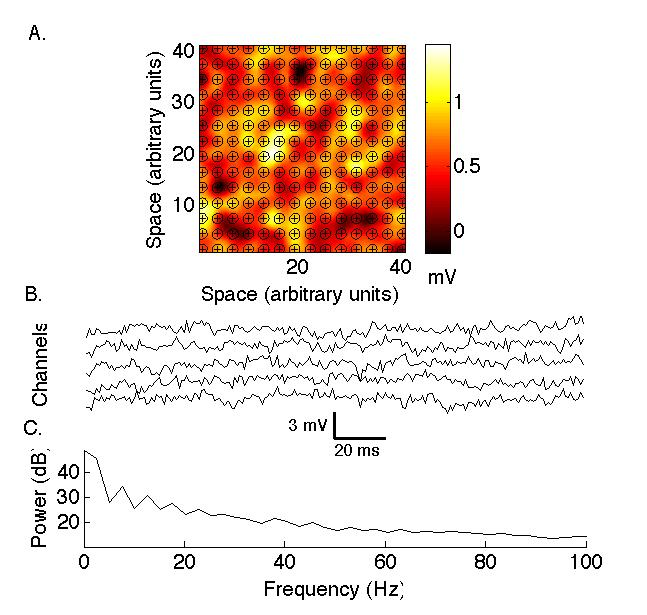
\includegraphics[scale=0.4]{./Graph/ExperimentFigure.jpg} 
	\end{center}
	\caption{Example of experimental design and model output. \textbf{A}. Example of the neural field with sensors. The centres of the sensors are shown by crossed and the sensor widths ($1/2$ height of Gaussian) are shown by the circles. \textbf{B} Example of data generated by the model through the observations. \textbf{C}. Power spectral density of the data generated by an observation showing the typical $1/f$ characteristic of iEEG.} \label{fig:FrequencyAnalysis} 
\end{figure}

\subsection{Spatial Frequency Analysis} In accordance with Section~\ref{SpectralAnalysisSection}, the spatial frequency of the field was used to confirm the spacing and width of the sensors was adequate to capture the significant dynamics of the field. Figure~\ref{} shows the spatial frequency of the field. The cut-off frequency, $\nu_c$, was taken to be \omg{??}, which corresponds to the \omg{??-3~dB} from the peak power. From equation~\ref{eq:MinimumSensorDistance}, this yielded a minimum sensor separation of \omg{??}. This confirms our separation was enough to prevent problems associated with aliasing.

The spatial frequency of the observations is shown in figure~\ref{}. The peak power of the spatial frequency of the observations was approximately $30$~dB. The cut-off frequency was taken to correspond to \omg{??} of the peak pwoer which was approximately $15$~dB. This provided a conservative The oversampling parameter $\rho=2$. From equation~\ref{}, this gives a minimum distance between basis functions of $2.7$ to satisfy Shannon's sampling criterion. \todo{maybe from Parham's derivation... From equation~\ref{} the width was calculated to be... or...}. The width of the basis functions was chosen such that they had sufficient overlap to represent the dynamic field.

\begin{figure}
	\begin{center}
		\subfigure[][]{
		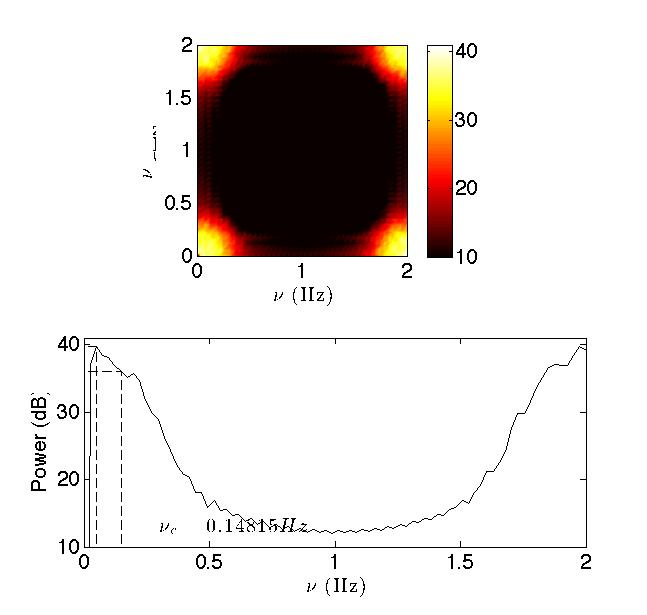
\includegraphics[scale=0.2]{./Graph/freq_analysis_filtered_field.jpg}} \subfigure[][]{
		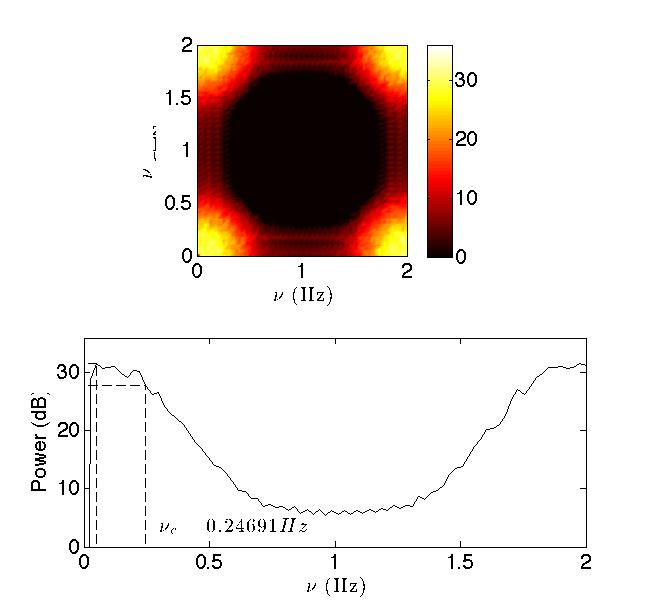
\includegraphics[scale=0.2]{./Graph/freq_analysis_field.jpg}} \subfigure[][]{
		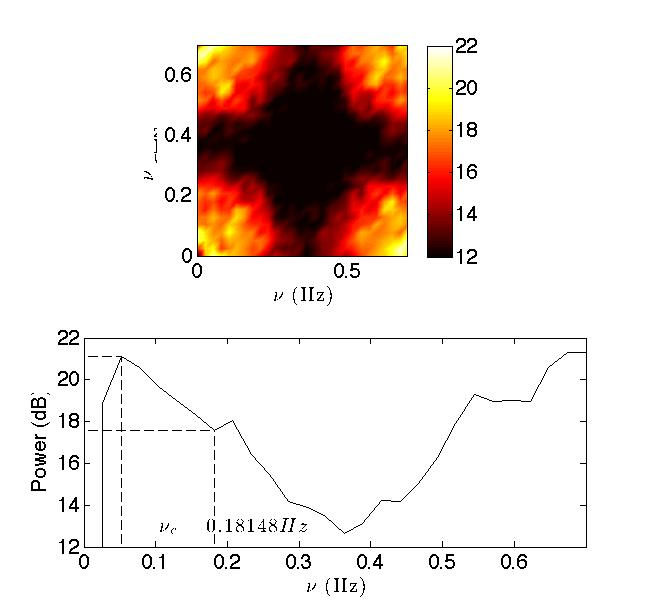
\includegraphics[scale=0.2]{./Graph/freq_analysis_sensor.jpg}} 
	\end{center}
	\caption{..... \textbf{A}. filtered field. \textbf{B} Field \textbf{C}. Power spectral density of the data generated by an observation showing the typical $1/f$ characteristic of iEEG.} \label{fig:ExampleFieldAndSensorsDataAndPSD} 
\end{figure}
Following this, the distance between basis function, $\Delta_b$, was set to $2.5$ and the basis function width, $\sigma_{\phi}^2$, was set to 3.6, 3.16 mm full width at half maximum. Analysis said 3.9 from Parham's derivation, but 3.6 still overlaps and allows more high frequency details to be represented.

\subsection{State and Parameter Estimates} To demonstrate the performance of the parameter and state estimation, $200$ realisations of the data were generated. Each realisation consisted of 300 ms of data and the estimation was applied to the final 200 ms, allowing the model to stabilise. The initial state and parameters were unknown to the estimator. The state estimates were evaluated by comparing the field reconstruction to the true field using the mean over time of the RMSE and standard deviation of the RMSE. The distribution of the state estimates are shown in figure~\ref{}. 

\section{Discussion}
\begin{itemize}
	\item if we don't know the frequency analysis or the system is marginally sampled or under-sampled, the best we can do is have the basis functions the same as the sensor kernel. \wtf{why wouldn't it be better to have, say, twice as many basis functions as we have sensors, at half the width?} 
	\item alternatives to frequency analysis are model selection... \wtf{This frequency analysis \emph{is} model selection. Maybe what's meant here is that other model selection approaches could be applied? Some sort of IC optimisation?} 
	\item the width of the connectivity basis functions \wtf{do you mean width of the kernel? I'm not sure about this - as the parameters increase the kernel width increases right? So maybe you mean the basis functions, but don't we estimate these widths from the frequency analysis?} here is known exactly. In practice we don't 
	\item the number of basis functions could be set higher to get a better representation of the field, however this is limited by computation complexity. \wtf{Unless you are going to specify the computational complexity, in terms of the number of basis functions, it might be better to say something like ``there is a relationship between the number of basis functions that represent the field and the computational complexity of the estimation algorithm - the more basis functions the longer it takes to estimate''} 
	\item Discuss the novelty of using the reduced model (BrainIDE) for creating patient specific models. \omg{hell yes. This should be front and centre!} 
	\item The size of the dentritic arbour is consistent in the cortex. \omg{?} 
	\item Spatial frequency of field and the relationship to the required density of electrodes/sensors required for estimation or to capture the required information without aliasing. 
	\item The flexibility of the approach 
	\item Combining this method with other to incorporate longer range hetrogeneous connectivity. \omg{awesome} 
	\item The need for activity to perform estimation. \omg{To Learn You Must Perturb!} 
\end{itemize}

\section{Conclusion} 
\appendix 
\section{Discrete Time Model}\label{Time Discretization} To form the IDE neural field model a time discretization must be perform. We used a one-step Euler method where Eq.~\ref{FinalForm1} can be approximated by 
\begin{equation}
	\label{Euler Approximation} \frac{v\left( \mathbf{r},t+T \right) - v\left( \mathbf{r},t\right)}{T_s} = -\zeta v\left( \mathbf{r},t \right) + \int_\Omega {w\left( \mathbf{r}-\mathbf{r}' \right)f\left( {v\left( \mathbf{r}',t \right)} \right)d\mathbf{r}'} + u\left(\mathbf{r},t\right). 
\end{equation}
For clarity, we shall index time points in the discrete time form of the model using the subscript $t$ and the next time point as $t+1$. Rearranging Eq.~\ref{Euler Approximation} we get 
\begin{eqnarray}
	\label{Euler Approximation} v_{t+1}\left( \mathbf{r}\right) &=& v_t\left( \mathbf{r}\right) -T_s \zeta v_t\left( \mathbf{r}\right) + T_s \int_\Omega {w\left( \mathbf{r}-\mathbf{r}' \right)f\left( {v_t\left( \mathbf{r}'\right)} \right)d\mathbf{r}'} + T_s u_t\left(\mathbf{r}\right). 
\end{eqnarray}
The discrete time form of the model is 
\begin{equation}
	\label{Discrete Time Model1} v_{t+1}\left(\mathbf{r}\right) = \xi v_t\left(\mathbf{r}\right) + T_s \int_\Omega { w\left(\mathbf{r}-\mathbf{r}'\right) f\left(v_t\left(\mathbf{r}'\right)\right) d\mathbf{r}'} + T_s u_t\left(\mathbf{r}\right), 
\end{equation}
where $\xi = 1 - T \zeta$. 
\section{Numerical Simulation of IDE Model}\label{Space Discretization} To solve the intregro-difference equation in Eq.~\ref{Discrete Time Model1} we define the spatial aspect of the model on a regular square $i,j$ grid of neural masses, where the spatial step size $\Delta \mathbf{r}_i = \Delta \mathbf{r}_j = \Delta $ giving 
\begin{equation}
	\label{discrete space} v_{t+1}\left(\mathbf{r}_{ij}\right) = \xi v_t\left(\mathbf{r}_{ij}\right) + T_s \Delta^2 \sum_{i=1}^{i=I}{ \sum_{j=1}^{j=J}{ w\left( \mathbf{r}-\mathbf{r}_{ij}' \right)f\left( v_t\left( \mathbf{r}_{ij}'\right) \right)} } + T_s u_t\left(\mathbf{r}\right) + e_t(\mathbf{r}_{i,j}), 
\end{equation}
where $e_t(\mathbf{r}_{i,j}) \sim \mathcal{N}\left(0,\Sigma\right)$. We have used free boundary conditions and extended the spatial domain to alleviate problems associated with edge effects. 
\section{Reduction to Finite State-Space Model}\label{Simplifying Decomposition} Starting from Eq.~\ref{reduced continuous model} we multiply throughout by $\boldsymbol{\phi}(r)$ and integrate over the spatial domain $\Omega$ to get 
\begin{eqnarray}
	\label{ReducingState} \int_\Omega {\boldsymbol{\phi} \left(\mathbf{r}\right)\boldsymbol{\phi}^{\top}\left(\mathbf{r}\right) d\mathbf{r}} \mathbf{x}_{t+1} = T_s \int_\Omega {\boldsymbol{\phi} (\mathbf{r}) \boldsymbol{\theta}^{\top} \int_\Omega {\boldsymbol{\psi} \left(\mathbf{r}-\mathbf{r}'\right) f\left(\boldsymbol{\phi}^{\top}\left(\mathbf{r}'\right) \mathbf{x}_t \right)d\mathbf{r}'}d\mathbf{r}} - \xi\int_\Omega {\boldsymbol{\phi}(\mathbf{r})\boldsymbol{\phi}^{\top}(\mathbf{r})d\mathbf{r}} \mathbf{x}_t \\
	+ T_s \int_\Omega{\boldsymbol{\phi} \left(\mathbf{r}\right) u_t\left(\mathbf{r}\right)d\mathbf{r}} + \int_\Omega{\boldsymbol{\phi} \left(\mathbf{r}\right) e_t\left(\mathbf{r}\right)d\mathbf{r}}. 
\end{eqnarray}
Substituting Eq.~\ref{DefGamma} into Eq.~\ref{Poo} and cross-multiplying by $\boldsymbol{\Gamma}^{-1}$ gives 
\begin{eqnarray}
	\label{Homogeneous SS Model} \mathbf{x}_{t+1} = T_s\boldsymbol{\Gamma}^{ - 1}\int_\Omega {\boldsymbol{\phi}\left(\mathbf{r}\right) \int_\Omega {f\left(\boldsymbol{\phi}^{\top}\left(\mathbf{r}'\right)\mathbf{x}_t\right) \boldsymbol{\psi}^{\top} \left(\mathbf{r}-\mathbf{r}'\right)d\mathbf{r}'} d\mathbf{r}} \boldsymbol{\theta} - \xi \mathbf{x}_t \\
	+ \boldsymbol{\Gamma}^{-1}T_s \int_\Omega{\boldsymbol{\phi} \left(\mathbf{r}\right) u_t\left(\mathbf{r}\right)d\mathbf{r}} + \boldsymbol{\Gamma}^{-1} \int_\Omega{\boldsymbol{\phi}\left(\mathbf{r}\right)e_t\left(\mathbf{r}\right)d\mathbf{r}}. 
\end{eqnarray}
\section{Reduction to Finite State-Space Model}\label{Simplifying Decomposition} Starting from Eq.~\ref{reduced continuous model} we multiply throughout by $\boldsymbol{\phi}(r)$ and integrate over the spatial domain $\Omega$ to get 
\begin{eqnarray}
	\label{StartofReduction} \int_\Omega {\boldsymbol{\phi} \left(\mathbf{r}\right)\boldsymbol{\phi}^{\top}\left(\mathbf{r}\right) d\mathbf{r}} \mathbf{x}_{t+1} = T_s \int_\Omega {\boldsymbol{\phi} (\mathbf{r}) \boldsymbol{\theta}^{\top} \int_\Omega {\boldsymbol{\psi} \left(\mathbf{r}-\mathbf{r}'\right) f\left(\boldsymbol{\phi}^{\top}\left(\mathbf{r}'\right) \mathbf{x}_t \right)d\mathbf{r}'}d\mathbf{r}} - \xi\int_\Omega {\boldsymbol{\phi}(\mathbf{r})\boldsymbol{\phi}^{\top}(\mathbf{r})d\mathbf{r}} \mathbf{x}_t \\
	+ T_s \int_\Omega{\boldsymbol{\phi} \left(\mathbf{r}\right) u_t\left(\mathbf{r}\right)d\mathbf{r}} + \int_\Omega{\boldsymbol{\phi} \left(\mathbf{r}\right) e_t\left(\mathbf{r}\right)d\mathbf{r}}. 
\end{eqnarray}
Substituting Eq.~\ref{DefGamma} into Eq.~\ref{StartofReduction} and cross-multiplying by $\boldsymbol{\Gamma}^{-1}$ gives 
\begin{eqnarray}
	\label{Homogeneous SS Model} \mathbf{x}_{t+1} = T_s\boldsymbol{\Gamma}^{ - 1}\int_\Omega {\boldsymbol{\phi}\left(\mathbf{r}\right) \int_\Omega {f\left(\boldsymbol{\phi}^{\top}\left(\mathbf{r}'\right)\mathbf{x}_t\right) \boldsymbol{\psi}^{\top} \left(\mathbf{r}-\mathbf{r}'\right)d\mathbf{r}'} d\mathbf{r}} \boldsymbol{\theta} - \xi \mathbf{x}_t \\
	+ \boldsymbol{\Gamma}^{-1}T_s \int_\Omega{\boldsymbol{\phi} \left(\mathbf{r}\right) u_t\left(\mathbf{r}\right)d\mathbf{r}} + \boldsymbol{\Gamma}^{-1} \int_\Omega{\boldsymbol{\phi}\left(\mathbf{r}\right)e_t\left(\mathbf{r}\right)d\mathbf{r}}. 
\end{eqnarray}
\section{}\label{ColoredNoise} 
\newtheorem{lemma}{Lemma} 
\begin{lemma}
	Consider the zero-mean process $e_t\left(\mathbf r\right)$ with covariance as defined by (\ref{eq:FieldCovariance}) then 
	\begin{equation}
		\mathbf e_t=\boldsymbol{\Gamma}^{-1}\int_\Omega {\boldsymbol{\phi} ( \mathbf{r} )e_t( \mathbf{r} )d\mathbf{r}} \label{eq:AppendixWt} 
	\end{equation}
	is a vector valued, zero mean normally distributed white noise process with covariance 
	\begin{equation}
		\boldsymbol\Sigma_e =\mathbf{\Gamma}^{-1}\int_{\Omega}\int_{\Omega}\boldsymbol{\phi}\left(\mathbf r\right) \gamma\left(\mathbf r- \mathbf r' \right)\boldsymbol{\phi}\left(\mathbf r'\right)^{\top}d\mathbf r' d\mathbf r\mathbf{\Gamma}^{- \top} 
	\end{equation}
	\label{lemma:FieldCovariance} 
\end{lemma}
\section*{Proof} Equation (\ref{eq:AppendixWt}) is a linear function of $e_t(\mathbf r)$ and hence $\mathbf{e}_t$ is also normally distributed. The expected value of $\mathbf e_t$ is given by 
\begin{eqnarray}
	\mathbf E\left[ \mathbf e_t\right]&=& \mathbf{\Gamma}^{-1}\int_{\Omega}\boldsymbol\phi\left(\mathbf{r}\right)\mathbf E\left[e_t\left(\mathbf{r}\right)\right] d\mathbf{r} \nonumber \\
	&=&\mathbf 0 
\end{eqnarray}
The covariance of $\mathbf{e}_t$ is 
\begin{eqnarray}
	\mathbf{\Sigma}_e&=&\mathbf{\Gamma}^{-1}\mathbf E[\int_{\Omega}\boldsymbol{\phi}\left(\mathbf{r}\right)e_t\left(\mathbf{r}\right)d\mathbf{r} \int_{\Omega}\boldsymbol{\phi}\left(\mathbf{r}'\right)^{\top} e_t\left(\mathbf{r}'\right)d\mathbf{r}']\mathbf{\Gamma}^{- \top} \nonumber \\
	&=&\mathbf{\Gamma}^{-1}\int_{\Omega}\int_{\Omega} \boldsymbol{\phi}\left(\mathbf{r}\right) \mathbf E[e_t\left(\mathbf{r}\right)e_t\left(\mathbf{r}'\right)]\boldsymbol{\phi}\left(\mathbf{r}'\right)^{\top}d\mathbf{r}' d\mathbf r\mathbf{\Gamma}^{- \top} \nonumber\\
	&=&\mathbf{\Gamma}^{-1}\int_{\Omega}\int_{\Omega}\boldsymbol{\phi}\left(\mathbf r\right) \gamma\left(\mathbf r- \mathbf r' \right)\boldsymbol{\phi}\left(\mathbf r'\right)^{\top}d\mathbf r' d\mathbf r\mathbf{\Gamma}^{- \top} 
\end{eqnarray}
\section{Proof of \ref{eq:GaussianFT} and \ref{eq:WidthFrequencyRelationship} }\label{ap:FrequencyAnalysis}
Applying the \textit{n}-dimensional Fourier transform \cite{Arsac1966} to an \textit{n}-dimensional Gaussian centered at the origin yields
\begin{eqnarray}
 G(\boldsymbol \nu)&=&\int_{\mathcal R^n}\mathrm{exp}\left({-\frac{1}{\sigma_{\phi}^2} \mathbf r^\top\mathbf r}\right)\mathrm{exp}\left(-2\pi i\boldsymbol\nu^\top\mathbf r\right)d\mathbf r \nonumber \\
&=&\int_{\mathcal R^n}\mathrm{exp}\left(-\frac{1}{\sigma_{\phi}^2}\left[\mathbf r +\sigma_{\phi}\pi i \boldsymbol\nu\right]^\top\left[\mathbf r +\sigma_{\phi}\pi i \boldsymbol\nu\right]\right)d\mathbf r \nonumber \\
&\times& \mathrm{exp}\left(-\sigma_{\phi}^2\pi^2\boldsymbol\nu^\top \boldsymbol\nu\right)
\end{eqnarray}
and 
\begin{equation}\label{eq:IntegralOfGaussian}
\int_{\mathcal R^n}\mathrm{exp}\left(-\frac{1}{\sigma_{\phi}^2}\left[\mathbf r +\sigma_{\phi}\pi i \boldsymbol\nu\right]^\top\left[\mathbf r +\sigma_{\phi}\pi i \boldsymbol\nu\right]\right)d\mathbf r=(\pi\sigma_{\phi}^2)^{\frac{n}{2}}
\end{equation}
which gives another scaled  Gaussian 
\begin{equation}
   \boldsymbol\Phi(\boldsymbol\nu)=(\pi\sigma_{\phi}^2)^{\frac{n}{2}}\mathrm{exp}\left(-\sigma_{\phi}^2\pi^2\boldsymbol\nu^\top \boldsymbol\nu\right)
\end{equation}
substituting $\sigma_{\nu}^2=\frac{1}{\pi^2\sigma_{\phi}^2}$ gives 
\begin{equation}
\boldsymbol\Phi(\boldsymbol \nu)=\left(\frac{1}{\pi\sigma_{\nu}^2}\right)^{\frac{n}{2}}\mathrm{exp}\left(-\frac{1}{\sigma_{\nu}^2}\boldsymbol\nu^\top \boldsymbol\nu\right).
\end{equation}
and hence completing the proof. For 3 dB attenuation at $\boldsymbol\nu_c$ we need to set
\begin{eqnarray}
 |\boldsymbol\Phi(\boldsymbol\nu_c)|^2&=&\left(\frac{1}{\pi\sigma_{\nu}^2}\right)^{n}\mathrm{exp}\left(-\frac{2}{\sigma_{\nu}^2}\boldsymbol\nu_c^\top \boldsymbol\nu_c\right)\\
&=&\frac{1}{2}|\boldsymbol\Phi(\mathbf 0)|^2
\end{eqnarray}
solving for $\sigma_{\nu}^2$ we get
\begin{equation}
 \sigma_{\nu}^2=\frac{2\boldsymbol\nu_c^\top \boldsymbol\nu_c}{\ln 2 }.
\end{equation}

\section{Parameter Estimation Using Least Squares}\label{LeastSquaresAppendix} 
\begin{equation}
	\mathbf x_{t+1}=\mathbf{x}_{t}+T_s \mathbf{Q}(\mathbf{x}_t)\boldsymbol{\theta}-\zeta T_s\mathbf{x}_t+T_s\Gamma^{-1}\int_\Omega\boldsymbol{\phi}(\mathbf r)\varepsilon_t(\mathbf r)d\mathbf r \label{eq:statespacemodel} 
\end{equation}
where the matrix $\mathbf Q_{n_x \times n_{\boldsymbol{\theta}}}(\mathbf x_t)$ is defined as 
\begin{equation}
	Q_{n_x \times n_{\boldsymbol{\theta}}}=\Gamma^{-1}\int_\Omega\boldsymbol{\phi}(\mathbf r)\int_\Omega f(\boldsymbol{\phi}^\top(\mathbf r')\mathbf x_t)\mathbf{\psi}^\top(\mathbf r-\mathbf r')d\mathbf r'd\mathbf r 
\end{equation}
and $T_s$ is the sampling period. Least Square method can be used as (\ref{eq:statespacemodel}) is linear in parameters. At each time instant we have 
\begin{eqnarray}
	\mathbf x_{1}&=&\mathbf x_{0}+T_s \mathbf Q(\mathbf x_0) \boldsymbol{\theta}-\zeta T_s\mathbf x_0+T_s\mathbf e_0 \nonumber \\
	\mathbf x_{2}&=&\mathbf x_{1}+T_s \mathbf Q(\mathbf x_1) \boldsymbol{\theta}-\zeta T_s\mathbf x_1+T_s\mathbf e_1\nonumber\\
	&\vdots& \nonumber\\
	\mathbf x_{n}&=&\mathbf x_{n-1}+T_s \mathbf Q(\mathbf x_{n-1}) \boldsymbol{\theta}-\zeta T_s\mathbf x_{n-1}+T_s\mathbf e_{n-1} 
\end{eqnarray}
in matrix form 
\begin{equation}
	\left[
	\begin{array}{cccc}
		\mathbf x_{1}\\\mathbf x_{2}\\\vdots\\\mathbf x_{n}
	\end{array}
	\right] -\left[
	\begin{array}{cccc}
		\mathbf x_{0}\\\mathbf x_{1}\\\vdots\\\mathbf x_{n-1}
	\end{array}
	\right] =T_s\left[
	\begin{array}{cc}
		\mathbf Q(\mathbf x_0)&-\mathbf x_{0}\\\mathbf Q(\mathbf x_1)&-\mathbf x_{1}\\\vdots\\
		\mathbf Q(\mathbf x_{n-1})&-\mathbf x_{n-1}
	\end{array}
	\right] \left[
	\begin{array}{cc}
		\boldsymbol{\theta} \\
		\zeta
	\end{array}
	\right]+T_s \left[
	\begin{array}{cccc}
		\mathbf e_0\\\mathbf e_1\\\vdots\\\mathbf e_{n-1}
	\end{array}
	\right] 
\end{equation}
or in compact form we have 
\begin{equation}
	\mathbf Z=\mathbf X \mathbf W+\boldsymbol \xi 
\end{equation}
where 
\begin{equation}
	\mathbf Z=\left[
	\begin{array}{cccc}
		\mathbf x_{1}-\mathbf x_{0}\\
		\mathbf x_{2}-\mathbf x_{1}\\\vdots\\
		\mathbf x_{n}-\mathbf x_{n-1}
	\end{array}
	\right],\quad \mathbf X=T_s\left[
	\begin{array}{cccc}
		\mathbf Q(\mathbf x_0)&-\mathbf x_{0}\\
		\mathbf Q(\mathbf x_1)&-\mathbf x_{1}\\\vdots\\
		\mathbf Q(\mathbf x_{n-1})&-\mathbf x_{n-1}
	\end{array}
	\right] ,\quad \mathbf W=\left[
	\begin{array}{cc}
		\boldsymbol{\theta} \\
		\zeta
	\end{array}
	\right],\quad \boldsymbol \xi=T_s\left[
	\begin{array}{cccc}
		\mathbf e_0\\\mathbf e_1\\\vdots\\\mathbf e_{n-1}
	\end{array}
	\right] 
\end{equation}
using the method of Least Square $ \mathbf W$ can be estimated 
\begin{equation}
	\mathbf W\approx(\mathbf X^\top\mathbf X)^{-1}\mathbf X^\top\mathbf Z 
\end{equation}
\section{Parameters} 
\begin{tabular}
	{c|c} \hline\hline Symbol & Description \\
	\hline $v(\mathbf{r},t)$ & mean membrane potential \\
	$g(\mathbf{r},t)$ & average action potential rate \\
	$\mathbf{r}$ & spatial location \\
	$t$ & time (s) \\
	$h(t)$ & post-synaptic response kernel \\
	$\eta(t)$ & Heaviside function \\
	$\zeta$ & inverse synaptic time constant \\
	$w(\mathbf{r},\mathbf{r}')$ & spatial connectivity kernel \\
	$f(\mathbf{r},t)$ & firing function rate \\
	$u(\mathbf{r},t)$ & external input \\
	$\Omega$ & spatial domain \\
	$f_{max}$ & maximal firing rate \\
	$\varsigma$ & slope of sigmoidal activation function \\
	$v_0$ & firing threshold \\
	$\delta(t)$ & Dirac-delta function \\
	$D$ & Temporal differential operator \\
	$L$ & number of basis function and dimension of state vector \\
	$e(\mathbf{r},t)$ & field disturbance, covariance $\gamma$\\
	$m(\mathbf{r},\mathbf{r}')$ & sensor kernel, variance $\sigma_m^2$ \\
	$\epsilon(\mathbf{r}_n,t)$ & observation noise, covariance $\Sigma_\epsilon$ \\
	$y(\mathbf{r}_n,t)$ & obseration \\
	$n$ & sensor index $n=1,..,N$ \\
	$T$ & time step \\
	$\xi$ & time constant parameter \\
	$\mathbf{\phi(r)}$ & vector of Gaussian basis functions \\
	$\mathbf{x}_t$ & state vector at time $t$ \\
	$\mathbf{\psi}$ & vector of connectivity kernel basis functions \\
	$\theta$ & vector of connectivity kernel parameters \\
	$\Gamma$ & inner product of field basis functions \\
	$q()$ & state function \\
	$k()$ & maps into to discrete state of input function \\
	$\mathbf{e}_t$ & state disturbance, covariance $\Sigma_e$ \\
	$\mathbf{C}$ & observation matrix \\
	$V(\nu)$ & Spectrum of the dynamic field \\
	$\nu$ & Spatial frequency \\
	$\nu_c$ & Spatial cut-off frequency \\
\end{tabular}
\begin{tabular}
	{c|c} \hline\hline Symbol & Description \\
	\hline $\Delta_s$ & Distance between adjacent sensors \\
	$\rho$ & Over-sampling parameter \\
	$\Delta_b$ & Distance between field basis functions \\
	$\sigma_{nu}^2$ & Variance of FT of Gaussian basis function \\
	$\sigma^2$ & Spatial variance of Gaussian in spatial domain \\
	$\hat{\mathbf{x}}$ & State estimate \\
	$\chi$ & Matrix of sigma vectors \\
	$\hat{\mathbf{x}}_t^{f-}$ & Forward \emph{a priori} estimate \\
	$\hat{\mathbf{x}}_t^f$ & Forward \emph{a posteriori} estimate \\
	$\hat{\mathbf{x}}_t^{b-}$ & Backward \emph{a priori} estimate \\
	$\hat{\mathbf{x}}_t^{b}$ & Backward \emph{a posteriori} estimate \\
	$P^f_t$ & Forward \emph{a posteriori} covariance matrix \\
	$P^{f-}_t$ & Forward \emph{a priori} covariance matrix \\
\end{tabular}
\section*{References} 
\bibliographystyle{unsrt} 
\bibliography{BrainIDE}

% \begin{thebibliography}{10}
% \bibitem{book1} Goosens M, Rahtz S and Mittelbach F 1997 {\it The \LaTeX\ Graphics Companion\/} 
% (Reading, MA: Addison-Wesley)
% \bibitem{eps} Reckdahl K 1997 {\it Using Imported Graphics in \LaTeX\ } (search CTAN for the file `epslatex.pdf')
% \end{thebibliography}
\end{document}
